\section{Установка, настройка и тестирование интернет-радио на реальном хостинге}

Как только мы удостоверились, что наше интернет-радио работает стабильно и без ошибок, можем переходить к загрузке его на хостинг.

Был выбран VPS хостинг под управлением операционной системы Ubuntu Linux. После оплаты аренды, были получены данные для подключения к терминалу Linux по протоколу SSH.
\begin{figure}[H]
  \centering
  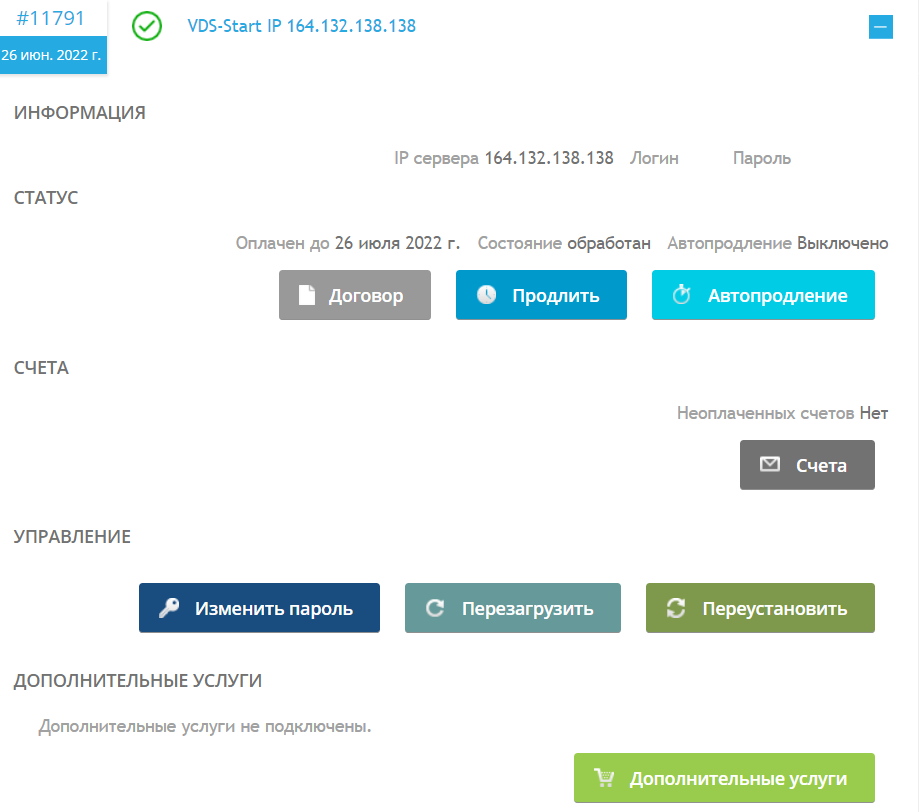
\includegraphics[interpolate, width=0.95\textwidth]{13}
  \caption{}
  \label{fig:13}
\end{figure}

Дальше, с помощью программного обеспечения Bitvise SSH Client, было произведено подключение к терминалу, и проделаны действия, аналогичные тем, что и при установке интернет-радио на локальном сервере.
\begin{figure}[H]
  \centering
  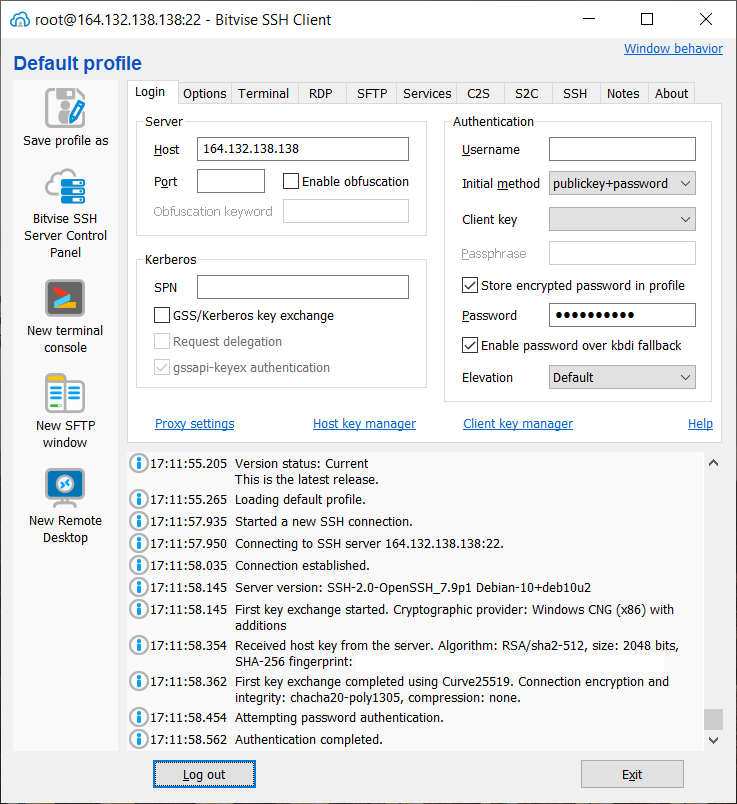
\includegraphics[interpolate, width=0.95\textwidth]{14}
  \caption{}
  \label{fig:14}
\end{figure}

\begin{figure}[H]
  \centering
  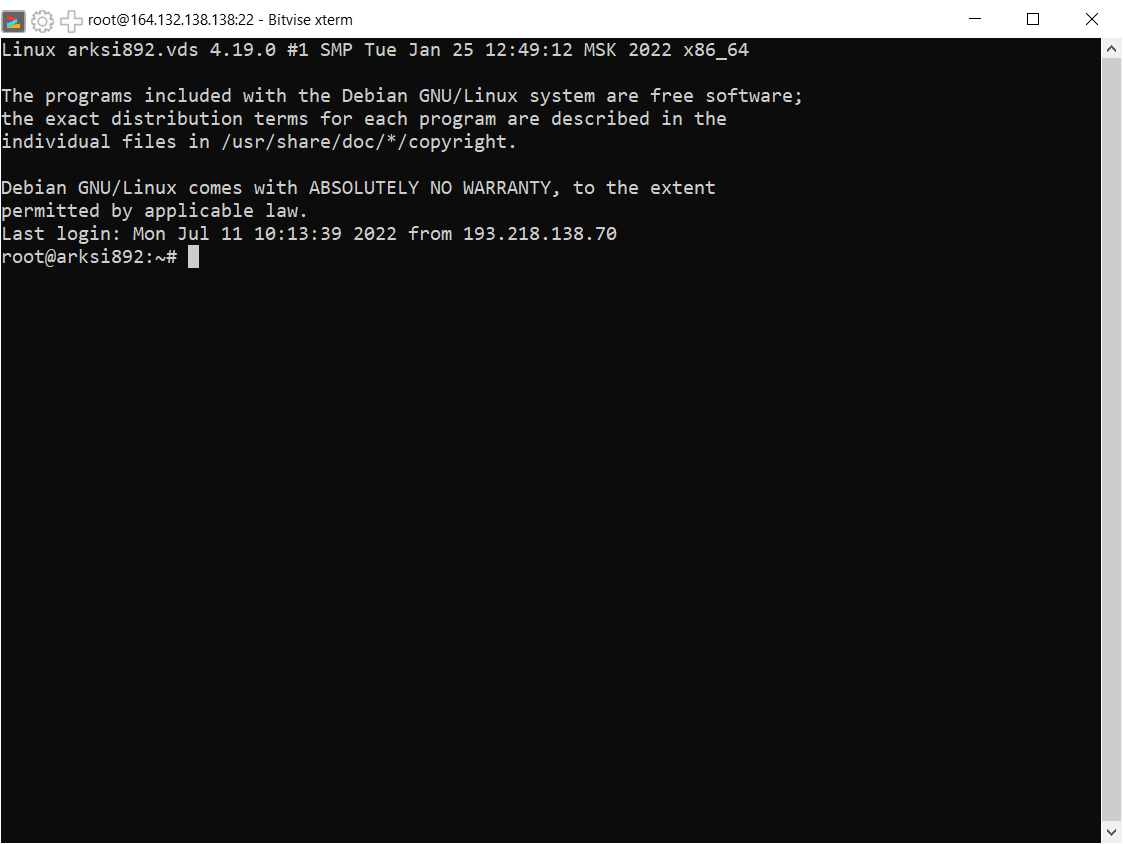
\includegraphics[interpolate, width=0.95\textwidth]{15}
  \caption{}
  \label{fig:15}
\end{figure}

По итогу, после настройки интернет-радио, мы получили и протестировали следующий результат.
\begin{figure}[H]
  \centering
  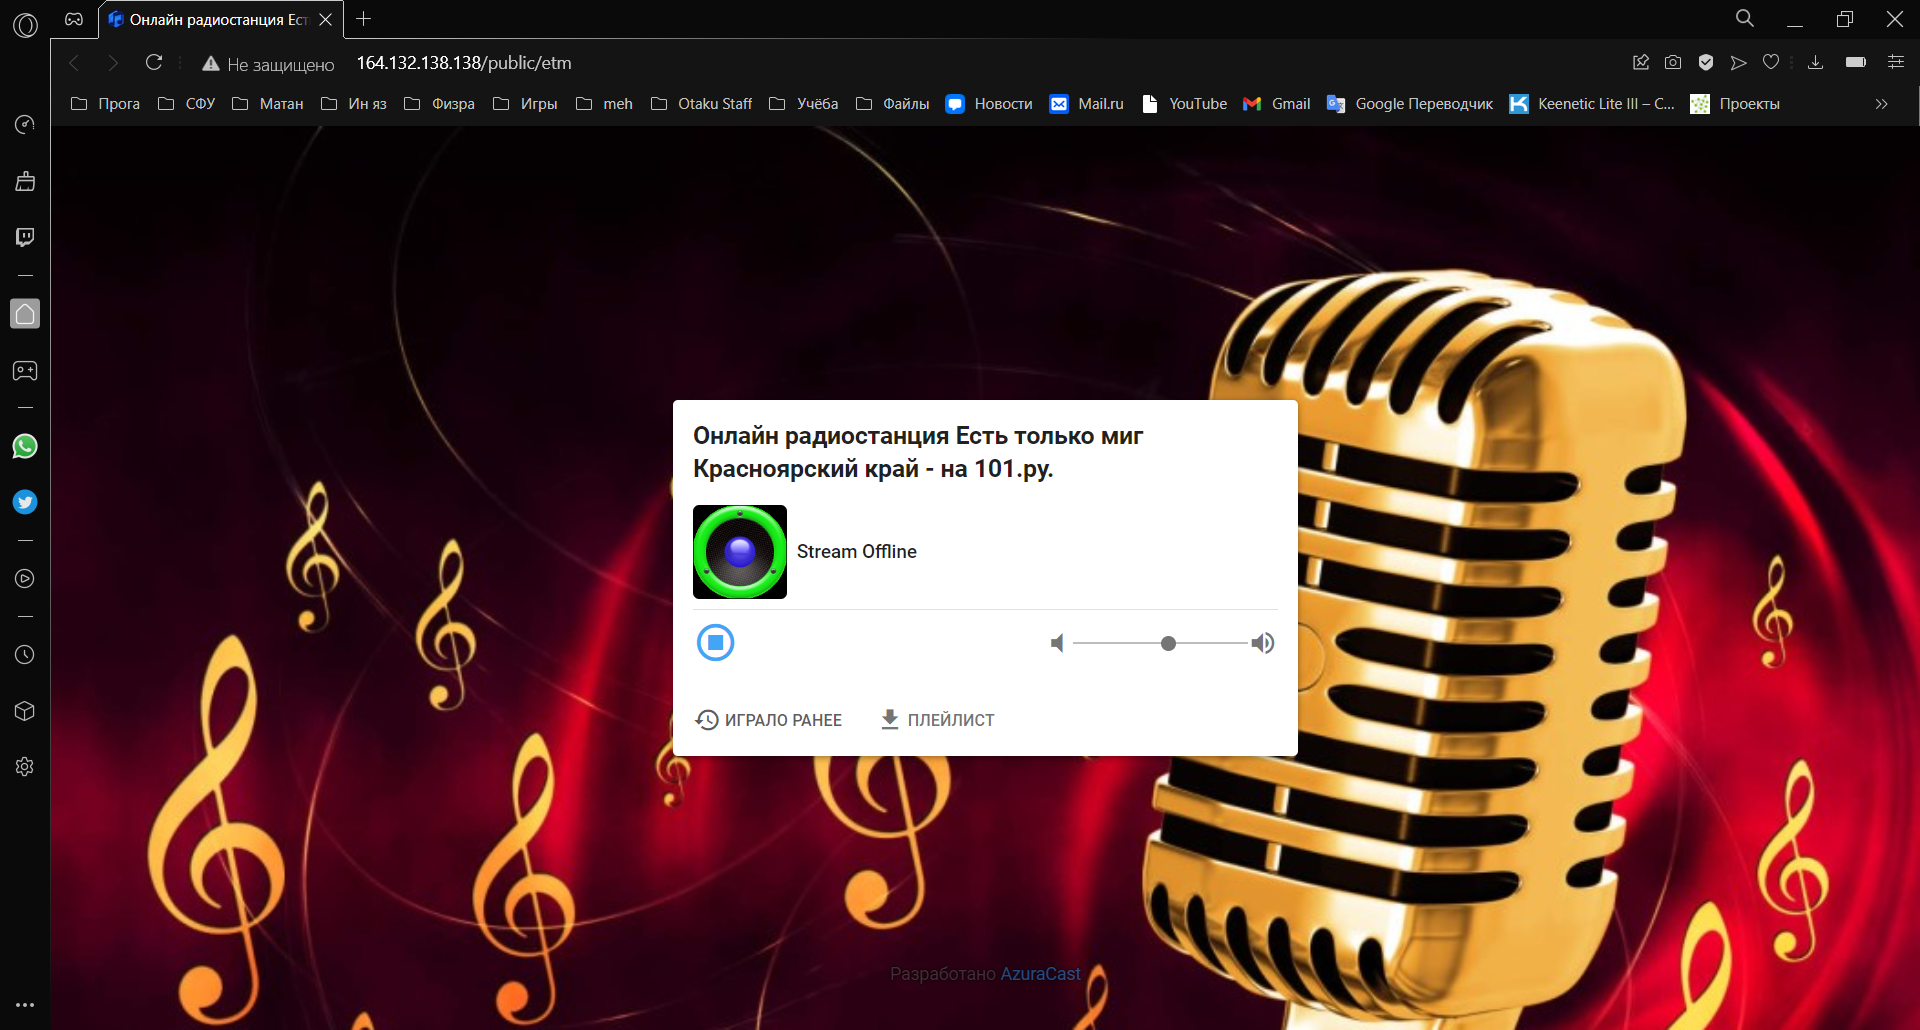
\includegraphics[interpolate, width=0.95\textwidth]{16}
  \caption{}
  \label{fig:16}
\end{figure}